%\chapter{Supercondensadores}
%TODO add asymetric reference
%TODO complejidad de las celdas de combustible
Almacenar energía eléctrica es uno de los mayores problemas a la hora de diseñar sistemas electrónicos móviles o estacionarios, los requerimientos varían de acuerdo a las necesidades de cada uno, en general es una competencia entre la densidad de energía (cuánta energía se puede almacenar) y la densidad de potencia (que tan rápido puede ser entregada la energía almacenada). Para poner en perspectiva las tecnologías de almacenamiento de energía, existe el diagrama de Ragone (ver figura \ref{fig:ragone}). Las celdas de combustible (\textit{Fuel Cells}), entregan la mayor densidad de energía, pero son complicadas. Mientras que las baterías poseen mayor densidad de potencia, pierden capacidad con los ciclos de carga y descarga. Los supercondensadores van un paso más allá, aumentado la densidad de potencia y aportando mayor vida útil, entregando una nueva posibilidad a la hora de diseñar sistemas eléctricos, ya sea como fuente de energía por sí mismo, o en sistemas híbridos combinados con otras tecnologías \citep{Thounthong2009}.\\
La densidad de energía de un supercondensador comparada a la de un condensador convencional es varios órdenes de magnitud superior, a modo de comparación, generalmente se utilizan microfaradios (10$^{-6}$ Faradios), para medir la capacidad de un condensador convencional, mientras que en un supercondensador es común ver capacidades de decenas o centenas de Faradios.


\begin{figure}
	\centering
	\fbox{
		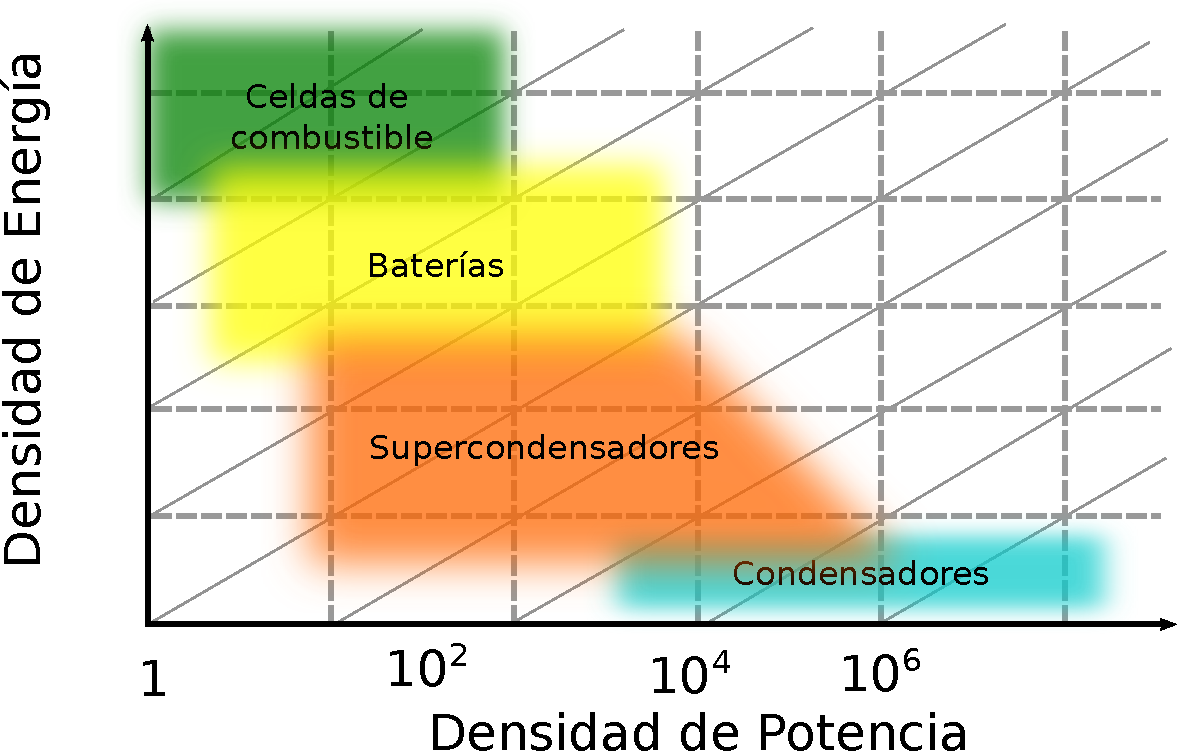
\includegraphics[width = 0.7\textwidth]{ragone.pdf}
	}
	\caption[Diagrama de Ragone]{El diagrama de Ragone compara diferentes tecnologías de almacenamiento de energía de acuerdo a su densidad de potencia y densidad de energía.}
	\label{fig:ragone}
\end{figure}

\subsection{El condensador ideal}
Generalmente un condensador se modela a través de dos placas paralelas separadas por un dieléctrico. Éste es definido por su capacitancia, la que refleja, \emph{grosso modo}, su capacidad de almacenar energía. Del modelo de placas paralelas se desprende la definición de capacitancia, $C$, como la razón entre la magnitud de carga en cada placa $Q$ y el voltaje entre los terminales $V$:

\begin{equation}
	C = \frac{Q}{V}
\end{equation}

La magnitud C es constante y depende de la construcción del condensador. Para fines prácticos, el condensador ideal como componente electrónico es modelado por la ecuación que relaciona la corriente\footnote{En estricto rigor, no hay corriente en el condensador, pues los electrones no ``saltan'' de una placa a otra, sólo se acumulan en una y se remueven en la otra, aparentando una corriente a través del dispositivo. La corriente en el condensador, es más bien una corriente de desplazamiento, pues es el campo eléctrico el que varía en el condensador.} con el voltaje entre los terminales del dispositivo. Considerando que $i = dq/dt$, entonces:

\begin{equation}
	i(t) = C \frac{dv(t)}{dt}.
\end{equation}
Esto quiere decir que la corriente es proporcional a la variación del voltaje en el tiempo.
En el caso de un proceso de carga y descarga a corriente constante, el voltaje variará linealmente, como lo muestra el gráfico de la figura \ref{fig:plot:charge-discharge_ideal_cap}.

\begin{figure}
	\centering
	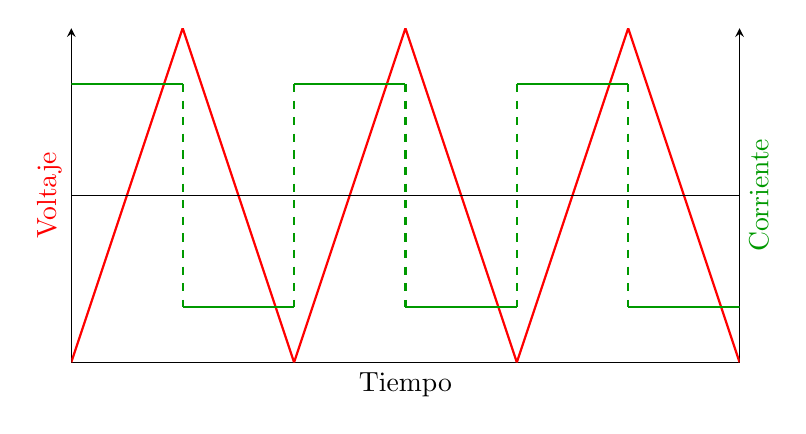
\begin{tikzpicture}
	% let both axes use the same layers
	\pgfplotsset{set layers, 	width=0.7\textwidth, height = 0.35\textwidth}
	
	\begin{axis}[
	scale only axis,
	axis y line=left, % the ’*’ avoids arrow heads
	axis x line*=bottom,
	xlabel=Tiempo,
	ylabel={\color{red} Voltaje},
	no markers,
	xmin=0,
	xmax=6,
	cycle list name=exotic,
	ticks=none,
	]
		\addplot [red, thick] table {
			A B
			%charge
			0 -1
			1  1
			
			2 -1
			3  1
			
			4 -1
			5  1
			
			%discharge
			1  1			
			2 -1
			
			3  1
			4 -1
			
			5  1
			6 -1
		};	
	\end{axis}
	\begin{axis}[
	scale only axis,
	axis y line=right,
	axis x line=none,
	ylabel={\color{green!60!black} Corriente},
	ymin = -1.5,
	ymax = 1.5,
	xmin = 0,
	xmax = 6,
	no markers,
	ticks=none,
	]
		\addplot [green!60!black, thick] table {
			A B
			0  1
			1  1
			
			1 -1
			2 -1
			
			2  1
			3  1
			
			3 -1
			4 -1
			
			4  1
			5  1
			
			5 -1
			6 -1	
		};
		\addplot [green!60!black, thick, dashed] table {
			A B
			1  1
			1 -1

			2  1
			2 -1
			
			3  1
			3 -1
			
			4  1
			4 -1
			
			5  1
			5 -1
		};
		\addplot [black] table {
			0  0
			6  0
		};
	\end{axis}
	\end{tikzpicture}
	\caption{Carga y descarga de un condensador ideal a corriente constante.}
	\label{fig:plot:charge-discharge_ideal_cap}
\end{figure}

\subsection{El condensador real}
%TODO agregar electrolito no acuoso
Un condensador ideal almacenaría una cierta cantidad de energía al cargarse y la entregaría totalmente en la descarga sin ninguna disipación, es decir, tendría una eficiencia del 100\%. Éste podría soportar cualquier amplitud de voltaje aplicado, o cargarse y descargarse por una corriente cuan grande se desee.  Sin embargo, en la vida real, los condensadores sí disipan energía, poseen voltajes de operación acotados y corrientes máximas de carga y descarga. Todo esto depende del diseño de cosntrucción y de los materiales empleados.\\
El voltaje máximo de operación de un condensador convencional dieléctrico, es determinado por la tensión de ruptura del material\footnote{Voltaje en el cual se pierden las propiedades dieléctricas del material, provocando cortocircuito al interior del dispositivo. Este está determinado por la fuerza dieléctrica y el espesor del material. En condensadores electrolíticos, la tensión de ruptura está determinada por otros mecanismos \citep{Yahalom1971}.}. En el caso de los supercondensadores, el voltaje máximo de carga depende fundamentalmente del electrolíto empleado, el que está limitado por potenciales límites de descomposición, como por ejemplo la descomposición del agua a 1.23 V para electrolitos acuosos.\\

\subsection{Resistencia en serie equivalente (ESR)}
Las imperfecciones en la construcción de los electrodos, y la resistencia intrínseca de los materiales utilizados, disipan energía durante la carga y descarga que se modela como una resistencia en serie con el condensador. Esto se ve reflejado como una caída de voltaje en los terminales del dispositivo (figura \ref{fig:plot:charge-discharge_esr}), disminuyendo la eficiencia de éste, esta caida de voltaje es:

\begin{equation}
	v = iR_{ESR}
\end{equation}

\begin{figure}
	\centering
	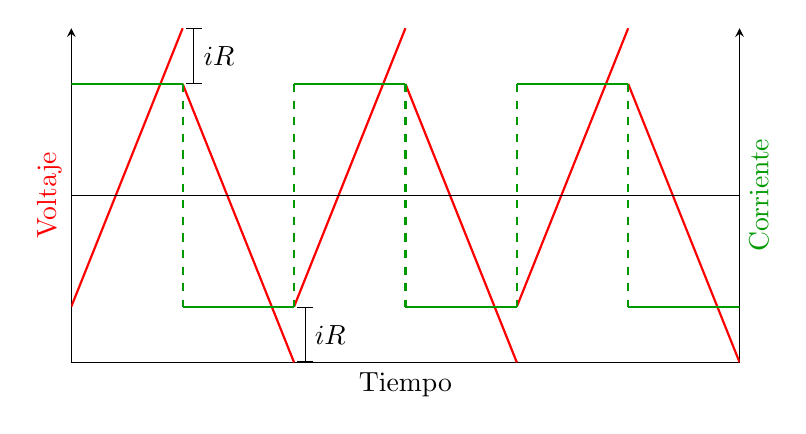
\begin{tikzpicture}
	% let both axes use the same layers
	\pgfplotsset{set layers, 	width=0.7\textwidth, height = 0.35\textwidth}
	
	\begin{axis}[
	scale only axis,
	axis y line=left, % the ’*’ avoids arrow heads
	axis x line*=bottom,
	xlabel=Tiempo,
	ylabel={\color{red} Voltaje},
	no markers,
	xmin=0,
	xmax=6,
	cycle list name=exotic,
	ticks=none,
	]
	\addplot [red, thick] table {
		A B
		%charge
		0 -0.8
		1  1.2
		
		2 -0.8
		3  1.2
		
		4 -0.8
		5  1.2
		
		%discharge
		1  0.8			
		2 -1.2
		
		3  0.8
		4 -1.2
		
		5  0.8
		6 -1.2
	};	
	\draw [arrows={|-|}] (axis cs:1.1,1.2) -- node[right]{$iR$} (axis cs:1.1,0.8);
	\draw [arrows={|-|}] (axis cs:2.1,-1.2) -- node[right]{$iR$} (axis cs:2.1,-0.8);
	\end{axis}
	\begin{axis}[
	scale only axis,
	axis y line=right,
	axis x line=none,
	ylabel={\color{green!60!black} Corriente},
	ymin = -1.5,
	ymax = 1.5,
	xmin = 0,
	xmax = 6,
	no markers,
	ticks=none,
	]
	\addplot [green!60!black, thick] table {
		A B
		0  1
		1  1
		
		1 -1
		2 -1
		
		2  1
		3  1
		
		3 -1
		4 -1
		
		4  1
		5  1
		
		5 -1
		6 -1	
	};
	\addplot [green!60!black, thick, dashed] table {
		A B
		1  1
		1 -1
		
		2  1
		2 -1
		
		3  1
		3 -1
		
		4  1
		4 -1
		
		5  1
		5 -1
	};
	\addplot [black] table {
		0  0
		6  0
	};
	\end{axis}
	\end{tikzpicture}
	\caption{Carga y descarga de un condensador evidenciando el efecto de una ESR.}
	\label{fig:plot:charge-discharge_esr}
\end{figure}



\subsection{Corriente de fuga (\emph{leakage current})}
%TODO agregar ejemplo
Entre los electrodos del condensador fluye una corriente no deseada cuando existe una diferencia de potencial (cuando el condensador está cargado), esta corriente descarga al condensador incluso si está desconectado. Esta imperfección es modelada como una resistencia en paralelo al condensador.

\subsection{Circuito equivalente}
El comportamiento de los condensadores reales (convencionales o electroquímicos), son modelados por un circuito equivalente, donde se introducen componentes que representan las imperfecciones del funcionamiento del condensador real.\\
En la figura \ref{fig:ciruitos_equivalente} se muestran dos circuitos equivalentes empleados para modelar un supercondensador. El de la figura \ref{fig:simple_randles} se denomina celda de Randles, y es el modelo más simple para un supercondensador. 

Con un modelo para el supercondensador se pueden encontrar los valores para cada componente de circuito mediante espectroscopía de impedancia electroquímica (EIS).
%\begin{figure}
%	\centering
%	\fbox{
%		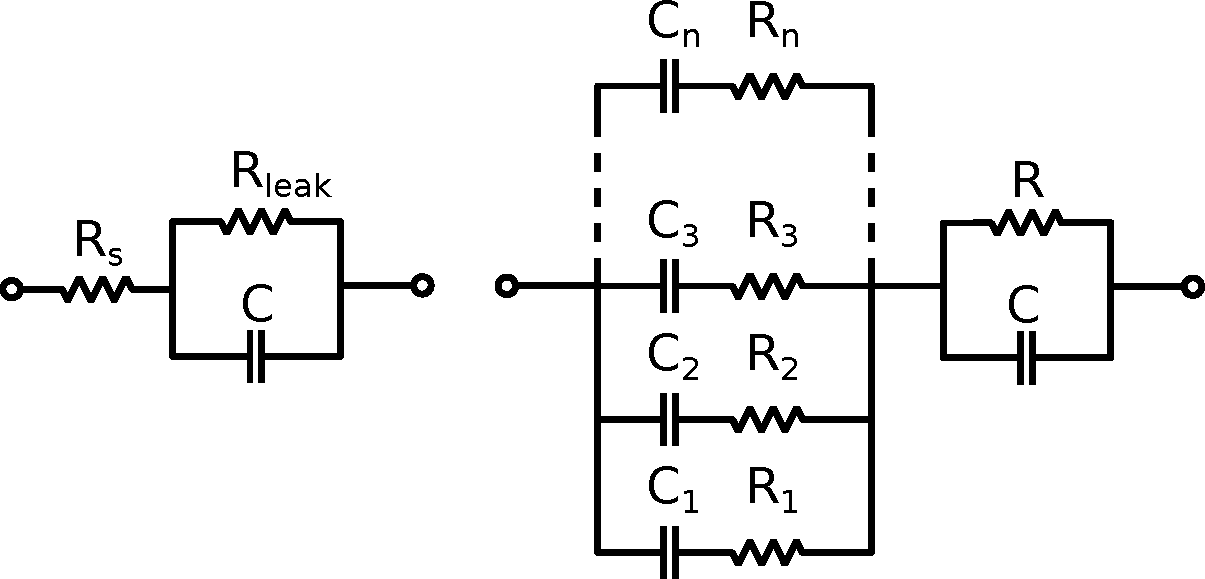
\includegraphics[width=0.7\textwidth]{equivalent_both.pdf}
%		}
%	\caption[Circuito equivalente]{Izquierda: Circuito equivalente sencillo. Derecha: Circuito equivalente complejizado \citep{Fletcher2014}.}
%	\label{fig:equiv_both}
%\end{figure}

\newcommand{\circuitscale}{1}
\begin{figure}
	\centering
	\begin{subfigure}{0.5\textwidth}
		\begin{circuitikz}[scale = \circuitscale, transform shape, font=\large]
			\draw (0,0)
			to [R=$R_s$,  o-] (2,0)
			to [short] (2,-1)
			to [C=$C$] (4,-1)
			to [short] (4,0)
			(2,0) to [short] (2,1)
			to [R=$R_{leak}$] (4,1)
			to [short] (4,0)
			to [short, -o] (5,0);
		\end{circuitikz}
		\caption{Circuito equivalente clásico.}
		\label{fig:simple_randles}
	\end{subfigure}\hfill
	\begin{subfigure}{0.5\textwidth}
			\begin{circuitikz}[scale = \circuitscale, transform shape, font=\large]
			\draw (0,0)
			to [R=$R_s$,  o-] (2,0)
			to [short] (2,-1)
			to [R=$R$] (4,-1)
			to [twoport, t=$W$] (6,-1)
			to [short] (6,0)
			(2,0) to [short] (2,1)
			to [C=$C_{dl}$] (6,1)
			to [short] (6,0)
			to [short, -o] (7,0);
			\end{circuitikz}
			\caption{Circuito equivalente Randles.}
			\label{fig:randles}
	\end{subfigure}
	\caption{Circuitos equivalentes.}
	\label{fig:ciruitos_equivalente}
\end{figure}

%%\begin{figure}
%	\centering
%
%%	\begin{circuitikz}[scale =\circuitscale, transform shape]
%%		\draw (1,0)
%%		to [short,o-] (2,0)
%%		to [C=$C_2$] (4,0)
%%		to [R=$R_2$] (6,0)
%%		to [short] (7,0)
%%		(2,0)
%%		to [short] (2,-2)
%%		to [C=$C_1$] (4,-2)
%%		to [R=$R_1$] (6,-2)
%%		to [short] (6,0)
%%		(7,0)
%%		to [short] (7,1)
%%		to [R=$R$] (9,1)
%%		to [short] (9,0)
%%		(7,0)
%%		to [short] (7,-1)
%%		to [C=$C$] (9,-1)
%%		to [short] (9,0)
%%		to [short,-o] (10,0);
%%		\draw[dashed] (2,0)
%%		to [short] (2,3)
%%		(6,3)
%%		to [short] (6,0);
%%		\draw (2,3)
%%		to [C=$C_n$] (4,3)
%%		to [R=$R_n$] (6,3);
%%	\end{circuitikz}
%	\caption{Circuito 1.}
%\end{figure}

\subsection{Supercondensadores}
Un supercondensador es un condensador que exhibe una capacitancia mucho mayor a la de un condensador normal (fácilmente 1000 veces mayor). No utilizan un material dieléctrico, si no un electrolito donde se forma una doble capa electrostática. Estos dispositivos están compuestos por dos electrodos de un material de gran área superficial específica, separados por una membrana permeable empapada en electrolíto (ver figura \ref{fig:edlc}). Si la capacidad del dispositivo surge de la separación de cargas en una doble capa electrostática de Helmholtz, se habla de condensadores de doble capa. Por otro lado, si la capacitancia surge de reacciones redox en los electrodos, se denominan pseudocondensadores, más aún, si la capacitancia surge de una doble capa y de reacciones redox, se tienen supercondensadores híbridos, donde generalmente, cada electrodo es de un material diferente.

\subsection{Doble capa electrostática de Helmholtz}
%TODO explicación doble capa
La gran densidad de energía de un supercondensador tiene que surgir de algún mecanismo de almacenamiento de cargas. A diferencia de las baterías, este mecanismo es puramente físico, pues no hay reacciones químicas en los electrodos, las cargas son separadas en lo que H. Helmholtz llamó \emph{Doble capa electrónica} \citep{Frackowiak2001}, así, los supercondensadores también son llamados EDLCs (del inglés \emph{Electric Double Layer Capacitor}), la cual consiste en

\begin{figure}[h!]
	\centering
	\fbox{
		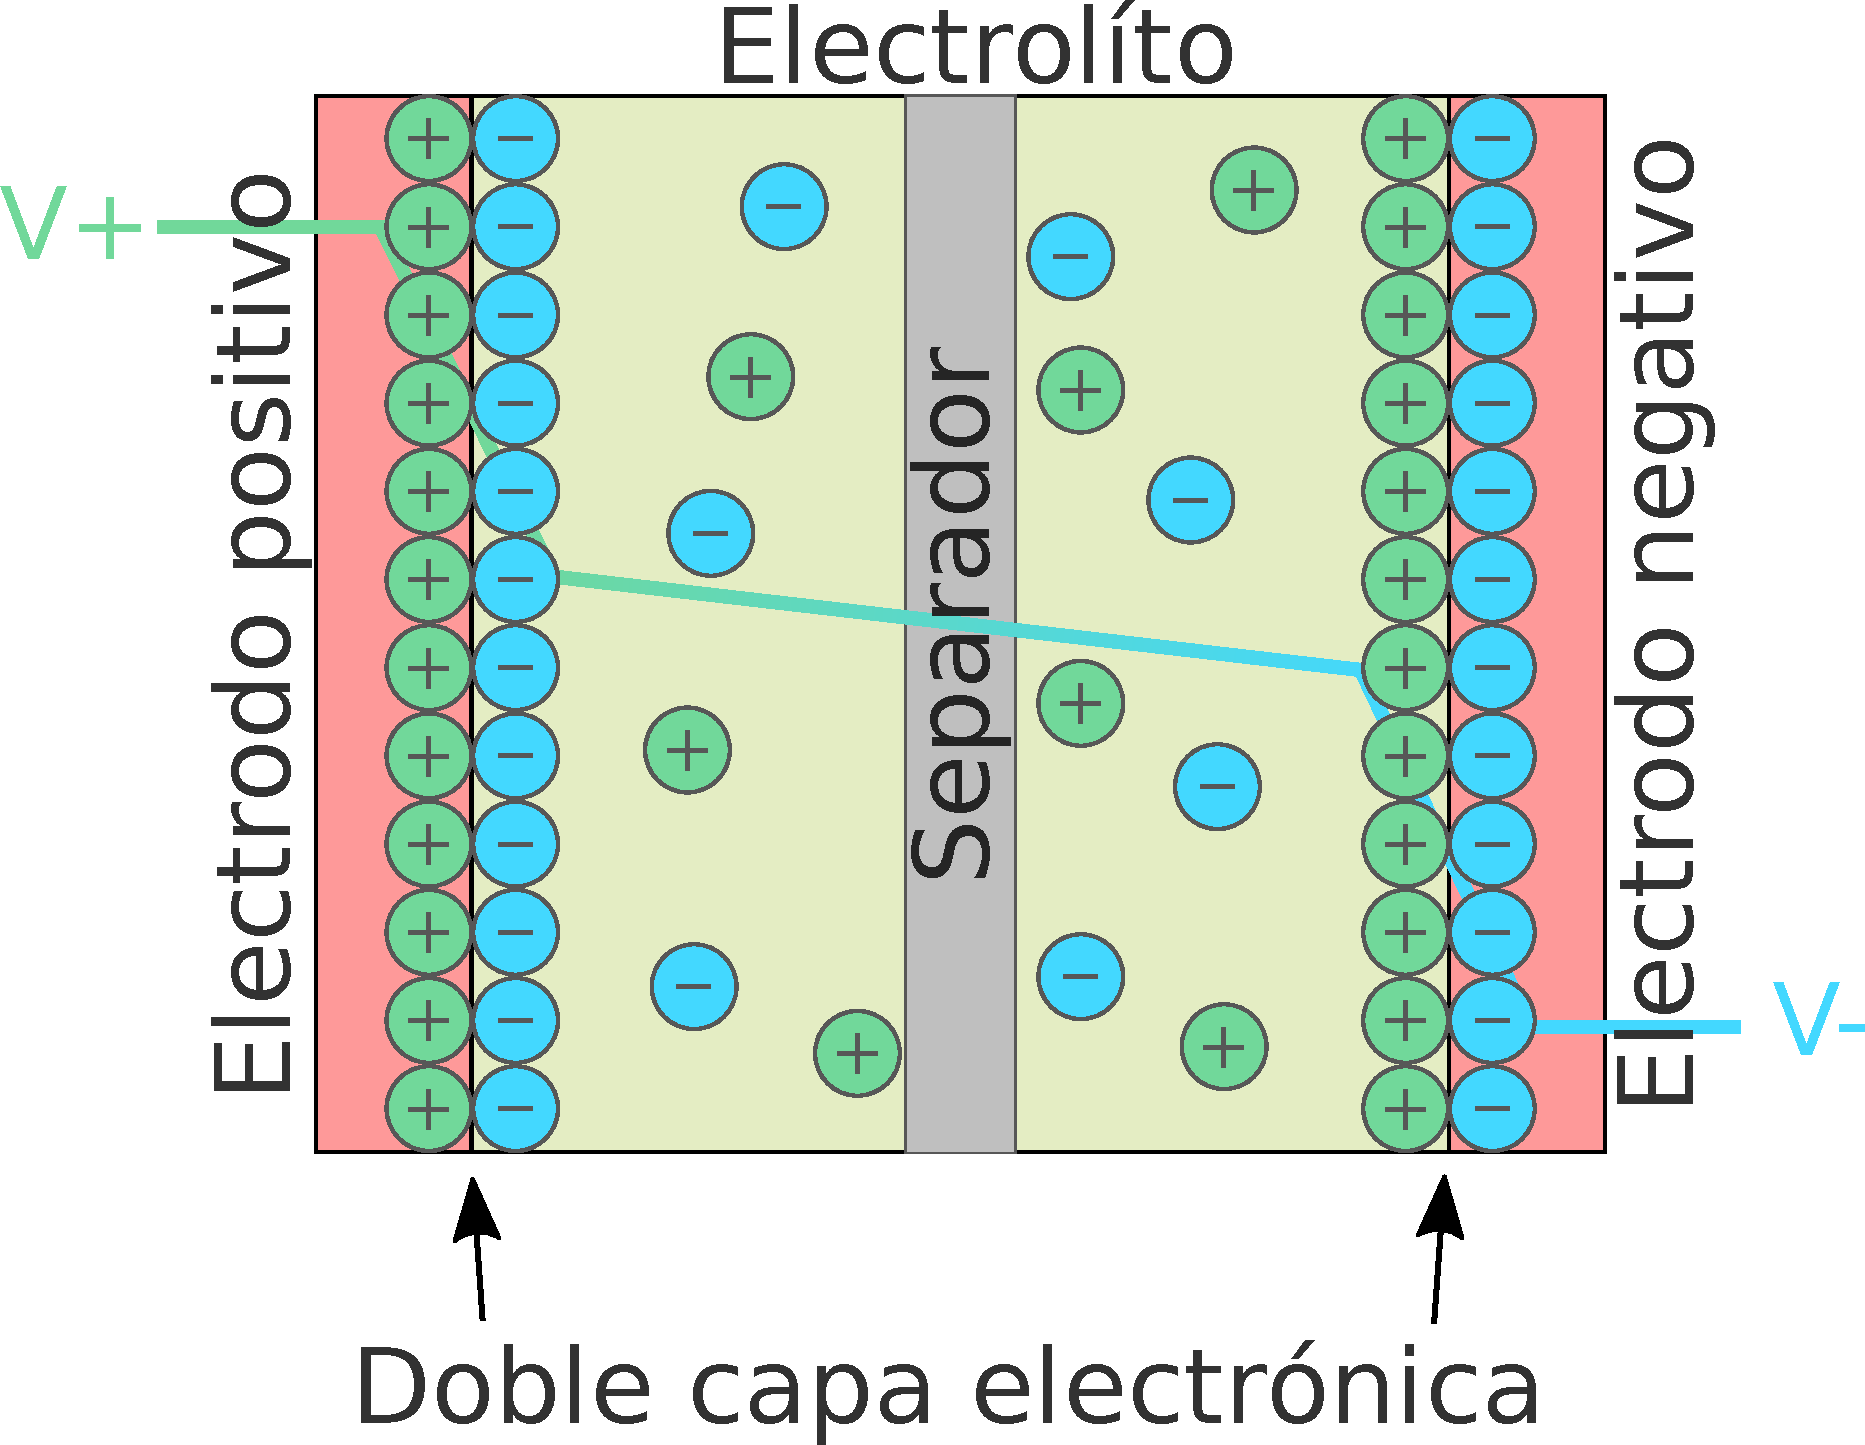
\includegraphics[width=0.7\textwidth]{edlc_schem.pdf}
		}
	\caption[Esquema de un supercondensador]{Esquema de un supercondensador mostrando una doble capa electrónica de Helmholtz en cada electrodo y el perfil del potencial eléctrico en él.}
	\label{fig:edlc}
\end{figure}

\subsection{Pseudocapacitancia}
Cuando en un supercondensador existe intercambio de electrones entre los electrodos y el electrolito (reacciones redox), se habla de pseudocapacitancia. El intercambio de electrones 


\subsection{Mediciones en supercondensadores}

\subsection{Voltametría cíclica}
%TODO explicar mejor
En una voltametría cíclica convencional, se varía el potencia entre los electrodos de manera lineal mientras se mide la corriente. Típicamente el barrido de voltaje se realiza entre dos voltajes fijos, y el recorrido se hace de ida y vuelta. Los parámetros importantes en la voltametría cíclica son: voltajes límite inferior y superior, velocidad de barrido.

La capacitancia específica $C_s$, puede ser calculada de la voltametría cíclica según la ecuación \ref{eq:cyclic_voltametry},

\begin{equation}\label{eq:cyclic_voltametry}
	C_{s} = \frac{\int_{V_1}^{V_2}i(v) \; dv}{2 \; \Delta V \; m \; \nu },
\end{equation}

donde $i$ y $v$ son la corriente y voltaje instantáneos, $V_1$ y $V_2$ los potenciales límite inferior y superior respectivamente, $\Delta V = V_2 - V_1 $, $m$ es la masa total del material activo en ambos electrodos, y $\nu$ la tasa de barrido. Esta ecuación corresponde a la carga total ($\int i\, dv / \nu$), dividida por la ventana de potencial $\Delta V$ y la masa, el factor $2$ surge de que la voltametría cíclica comprende tanto un ciclo de carga como uno de descarga.

\subsection{Espectroscopía de impedancia electroquímica}
Una señal sinusoidal (corriente o voltaje), de determinada amplitud y frecuencia, es aplicada en los terminales del dispositivo midiendo la respuesta de fase y corriente o voltaje según corresponda. La impedancia del sistema es caracterizada en un espectro de frecuencia, la que comúnmente es estudiado entre los mHz y los MHz. Una representación de los datos obtenidos es el gráfico de Nyquist, el cual consiste en un gráfico paramétrico con la frecuencia como parámetro, donde el eje de las abscisas corresponde a la parte real de la impedancia y las ordenadas a la parte imaginaria. Cualitativamente la forma de la curva obtenida sirve para asignar un circuito equivalente al dispositivo estudiado, sin embargo, también es posible calcular algunas cantidades, como por ejemplo la resistencia en serie equivalente.

\subsection{Carga y descarga cíclica}
%TODO explicar cantidad de ciclos
En este proceso la corriente es aplicada de forma constante para cargar el condensador hasta un potencial preestablecido, cuando dicho potencial es alcanzado, se aplica una corriente en sentido contrario para descargar el condensador hasta un potencial inferior predefinido. De las curvas de carga y descarga se puede determinar la capacitancia del condensador, y la resistencia en serie equivalente. Extendiendo la medición a miles de ciclos (hasta 10.000 ciclos), se puede determinar cómo será el comportamiento del dispositivo al pasar el tiempo.
De esta medición se puede calcular la capacitancia y la resistencia en serie equivalente.